\documentclass[10pt, a4paper]{article}

%\usepackage[paper=a4paper, left=1.5cm, right=1.5cm, bottom=1.5cm, top=3.5cm]{geometry}
\usepackage[paper=a4paper]{geometry}
\usepackage[latin1]{inputenc}
\usepackage[T1]{fontenc}
\usepackage[spanish]{babel}
\usepackage{indentfirst}
\usepackage{fancyhdr}
\usepackage{latexsym}
\usepackage{lastpage}
\usepackage[colorlinks=true, linkcolor=blue]{hyperref}
\usepackage{calc}
\usepackage{paralist}
\usepackage{caratula}
%\usepackage[plain,noline,linesnumberedhidden, noend]{algorithm2e}
%\usepackage[plain,noline,linesnumbered, noend]{algorithm2e}
\usepackage[plain,noline,noend]{algorithm2e}
\usepackage{graphicx}
\usepackage{caption}
\usepackage{subcaption}
\usepackage{amsmath}
\usepackage{float}
\usepackage{ulem}

\newcommand{\f}[1]{\text{#1}}
\newcommand{\call}[1] {\textsc{#1}}
\newcommand{\tab}[1]{\Indp \Indp #1 \Indm  \Indm}
\newcommand{\tabSpace}[1]{\Indp \Indp \; #1 \Indm \Indm \;}
\newcommand{\si}[2]{ {\bf si} (#1)\; \tab {#2} }
\newcommand{\sino}[1]{ {\bf sino}\; \tab {#1} }
\newcommand{\sinosi}[2]{ {\bf sino, si #1}\; \tab {#2} }
\newcommand{\mientras}[2] {  {\bf mientras} (#1) \; \tabSpace  {#2} }
\newcommand{\funcion}[3] { 	\KwSty{\call{#1}(#2)}\; \tabSpace  {#3} \KwSty{\call{Fin Funcion}} \newline }
\newcommand{\funcionConResultado}[4] {      \KwSty{\call{#1}(#2) $\rightarrow$ #3}\; \tabSpace  {#4} \KwSty{\call{Fin Funcion}} \newline }
\newcommand{\porcada}[3] { {\bf por cada } #1 {\bf en} #2 \; \tabSpace {#3} }
\newcommand{\para}[4] { {\bf para } #1 {\bf desde} #2 {\bf hasta} #3\; \{ \; \tab{#4}\}\; }
\newcommand{\paracada}[3] { {\bf para cada } #1 {\bf $\in$} #2 \; \tabSpace {#3} }
\newcommand{\devolver}[1] { {\bf devolver} #1\;}



\sloppy


\hypersetup{%
 % Para que el PDF se abra a pagina completa.
 pdfstartview= {FitH \hypercalcbp{\paperheight-\topmargin-1in-\headheight}},
 pdfauthor={C\'atedra de Algoritmos y Estructuras de Datos III - DC - UBA},
 pdfkeywords={Trabajo Pr\'actico 3},
 pdfsubject={}
}

\parskip=5pt % 10pt es el tama\~no de fuente

% Pongo en 0 la distancia extra entre itemes.
\let\olditemize\itemize
\def\itemize{\olditemize\itemsep=0pt}

% Acomodo fancyhdr.
\pagestyle{fancy}
\thispagestyle{fancy}
\addtolength{\headheight}{1pt}
\lhead{Base de Datos}
\rhead{TP2}
\cfoot{\thepage /\pageref{LastPage}}
\renewcommand{\footrulewidth}{0.4pt}

\author{Base de Datos, DC, UBA.}
\date{}
\title{}

\begin{document}

%Pagina de titulo e indice
\thispagestyle{empty}
\materia{Base de datos}
\submateria{TP2}
\titulo{}
\grupo{NN\_3}
\integrante{Sergio Gonz\'alez}{723/10}{sergiogonza90@gmail.com}
\integrante{Gino Scarpino}{392/08}{gino.scarpino@gmail.com}
\maketitle

\tableofcontents

\SetAlgoSkip{bigskip}
\NoCaptionOfAlgo
\DontPrintSemicolon
\SetAlFnt{\ttfamily}

\newpage

\section{Introducci\'on}

	\quad Es fundamental para cualquier motor de bases de datos, poseer un planificador para resolver consultas lo m\'as eficiente posible. Medir el costo de un m\'etodo de evaluaci\'on puede ser muy complejo, pero como se indica en el paper de Piatetsky-Shapiro, aproximadamente son las cantidad de operaciones de entrada y salida en disco que el motor realiza. Por eso mismo, se trata de minimizar estas operaciones.


\quad Una de las formas de poder minimizar estas operaciones, es conocer aproximadamente cual puede ser la distribuci\'on de un set de datos, y de esta forma poder estimar cuantas tuplas se obtendr\'a por el hecho de aplicar un filtro (WHERE) u otro que lo cumplan. El hecho de poder minimizar las tuplas resultantes que se obtendr\'an en una consulta, puede hacer que al momento de materializar la misma (por ejemplo en caso de tener que hacer un JOIN posterior) haga que las bajadas a disco de las tuplas se minimizen considerablemente.


\quad Si bien computar la distribuci\'on exacta de un set de datos puede ser muy costoso, existen m\'etodos con el cual se puede aproximar dichas distribuciones y de esa forma poder decidir cual es el mejor camino a seguir al momento de tener que resolver una consulta.




\section{Estimadores }

	\quad En este trabajo veremos tres estimadores, que los explicaremos a continuaci\'on:

\begin{itemize}
\item \textbf{Histograma Cl\'asico: } este estimador divide el rango de los valores en varios subrangos llamados \textit{buckets}. Contabiliza los cada valor aumentando la cantidad del \textit{bucket} correspondiente. Se basa fuertemente en estimar la probabilidad de un valor v con la cantidad total de elementos del \textit{bucket} correspondiente a ese v. Cuanto mayores subrangos haya, m\'ayor va a ser la precisi\'on para determinar la frecuencia del valor y de ah\'i estimar su selectividad. \\

\item \textbf{Pasos Distribuidos: } estimador inventado por Piatetsky-Shapiro. Al igual que en los histogramas cl\'asicos, usa el concepto de \textit{bucket} pero en vez de usar un ancho (rango) fijo para cada bucket, la cantidad de elementos en un \textit{bucket} est\'a determinada por la altura del mismo. Depende de la cantidad de \textit{buckets} que se desea, dividiendo la cantidad total de elementos (tuplas) por esa cantidad se obtiene la altura.\\

\item \textbf{Estimador Propio: } Nos basamos en el histograma cl\'asico pero introducimos una peque\~na mejora para ciertos casos (m\'as adelante se ver\'a en los an\'alisis de los testeos). Realizamos un histograma cl\'asico, luego detectamos una cantidad arbitraria de buckets con mayor cantidad de elementos y dividimos su rango en la mitad creando dos nuevos buckets. Cabe destacar que esto no significa que al dividir el rango en la mitad, se dividan la cantidad de elementos en la mitad. Para poder realizar esto, utilizamos un arreglo que mantiene informaci\'on espec\'ifica de cada \textit{bucket}, su rango. Notamos que la desventaja con respectoa  los otros dos estimadores es que en cada subdivisi\'on de un buckets necesitamos realizar una consulta a la base de datos para determinar cu\'antos elementos van en cada nuevo bucket. Para este trabajo, creamos el histograma cl\'asico con la mitad de buckets pasados como par\'ametro. Vamos dividiendo buckets que tengan el m\'aximo n\'umero de elementos hasta llegar a la cantidad de buckets indicada por par\'ametro.

\end{itemize}

	
\newpage

\section{An\'alisis de m\'etodos}

	\subsection{Distribuciones utilizadas}
	
		\subsubsection{Distribucion normal (Ejemplos)}	
		
			La distribuci\'on normal es una de las distribuciones que mas aparece en la vida real. A continuaci\'on se presentan 2 ejemplos de la misma.
	
	\subsubsection*{Altura de una persona}
	
		Es ampliamente conocido que las caracter\'isticas morfol\'ogicas de individuos, tales como la estatura, siguen el modelo normal en todo el mundo. En general, se puede pensar la altura de las personas suele estar entre 1-70 y 1.75 metros, debido a que en la mayor\'ia de los casos es as\'i. Es minor\'ia las personas que midan menos de 1.50, y a la vez no hay tampoco demasiadas personas que superen los 2 metros. Haciendo un muestreo poblacional y realizando un histograma del mismo se puede visualizar esta intuici\'on.
		
\begin{figure}[H]
  \begin{center}
    %\includegraphics[scale=.41,angle=-90]{imgenes/normal_ejemplo1.png}
    \includegraphics[scale=.40]{imagenes/normal_ejemplo1.png}
    \caption{Histograma altura} 
    \label{fig:normal_ejemplo1}
  \end{center}
\end{figure}		
		
Se puede ver como para el muestreo realizado, la mayor\'a de las personas caen en la altura entre 1.70 y 1.80 metros, dando como resultado aproximadamente, una normal con media 1,75 y desv\'io standard 0.64.

\newpage

	\subsubsection*{IQ de una persona}
	
		Otro ejemplo muy conocido es el coeficiente intelectual de las personas, conocido como IQ. Seg\'un el siguiente ranking, vemos que una inteligencia normal deber\'ia estar entre los 90 y los 109 de coeficiente intelectual. Por lo que es de esperar que la mayor parte de la poblaci\'on este en este promedio.
\newline

\begin{tabular}{| l | l |}
\hline
IQ Range & Clasificaci\'on \\
\hline
130 o mas & Muy Superior \\
\hline
120\--129	& Superior \\
\hline
110\--119	& Arriba del promedio \\
\hline
90\--109	& Promedio \\
\hline
80\--89	& Abajo del Promedio \\
\hline
70\--79	& L\'imite \\
\hline
69 o menos & Extremadamente bajo \\
\hline
\end{tabular}
\newline

\noindent 
Veamos un histograma sobre el muestreo del IQ de los individuos de una poblaci\'on. 


\begin{figure}[H]
  \begin{center}
    %\includegraphics[scale=.41,angle=-90]{imgenes/normal_ejemplo1.png}
    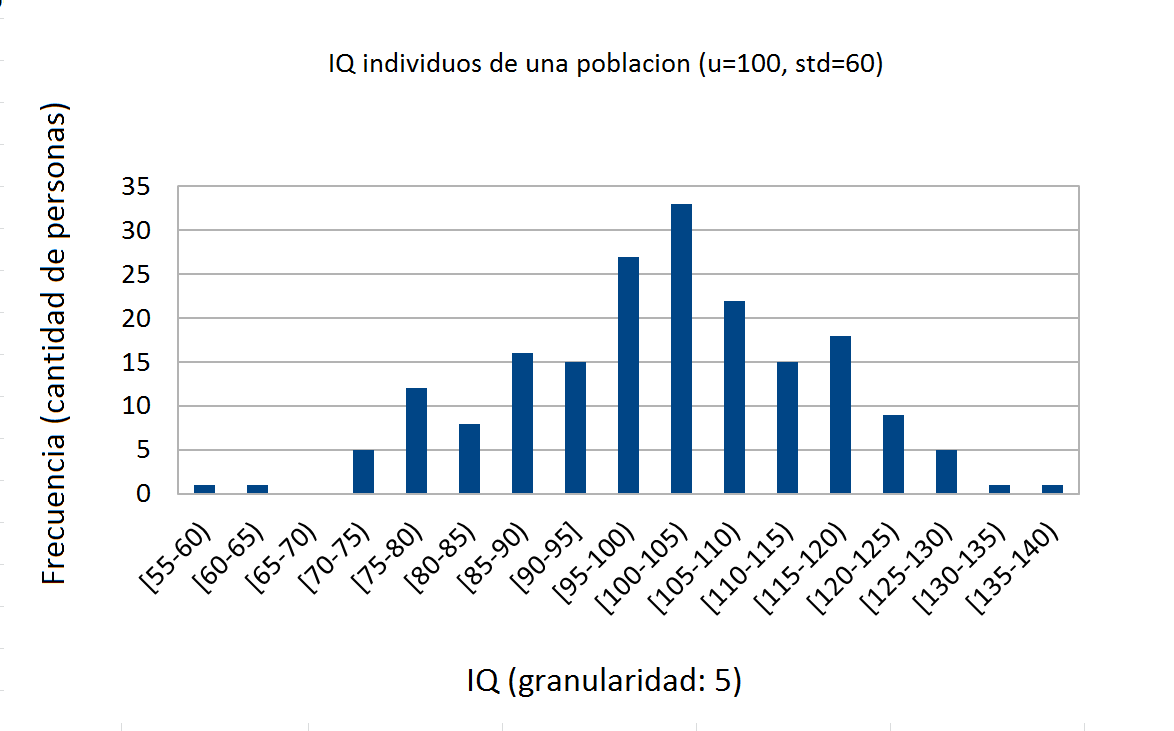
\includegraphics[scale=.40]{imagenes/normal_ejemplo2.png}
    \caption{Histograma IQ} 
    \label{fig:normal_ejemplo2}
  \end{center}
\end{figure}	

En la figura \ref{fig:normal_ejemplo2}, podemos un ver como, efectivamente, la mayor\'ia de la poblaci\'on se centra en un IQ de 100, con una desv\'io al rededor de 20.		
		
		\subsubsection{Distribucion uniforme (Ejemplos)}	
		
				La distribucion uniforme es una de las mas conocidas, y como la nomal, una de las mas presentes en la realidad.
	Esta distribucion es muy simple, basicamente plantea que si tenemos un espacio muestral $S=\{m_1, m_2, ... ,m_n\}$, $(\forall m_i \in S$,  $P(m_i)=1/n)$, osea, todos los sucesos tiene la misma probabilidad de ocurrir. 
			
	El ejemplo mas clasico para entender esa distribucion, es el lanzamiento de un dado de 6 caras (no cargado), en onde $S = \{1, 2, 3, 4, 5, 6\}$ y cada elemento tiene la misma probabilidad de salir, osea $1/6$.
			
\subsubsection*{Tiempo de espera de un colectivo}

	Otro ejemplo un poco mas interesante, es si tomamos un rango de tiempo, y medimos el tiempo de espera de un colectivo en ese rango de tiempo. Si bien este ejemplo dependera mucho de sobre que linea de colectivo hagamos el muestreo, se puede tomar un rango en particular en el cual sabemos que el tiempo de espera no sera mayor o menor a eso. A continuacion se presenta un histograma sobre un dataset sobre los tiempos de cierto colectivo en el rango de 5 minutos a 30 minutos.

\newpage					
	\begin{figure}[H]
	  \begin{center}
	    %\includegraphics[scale=.41,angle=-90]{imgenes/normal_ejemplo1.png}
	    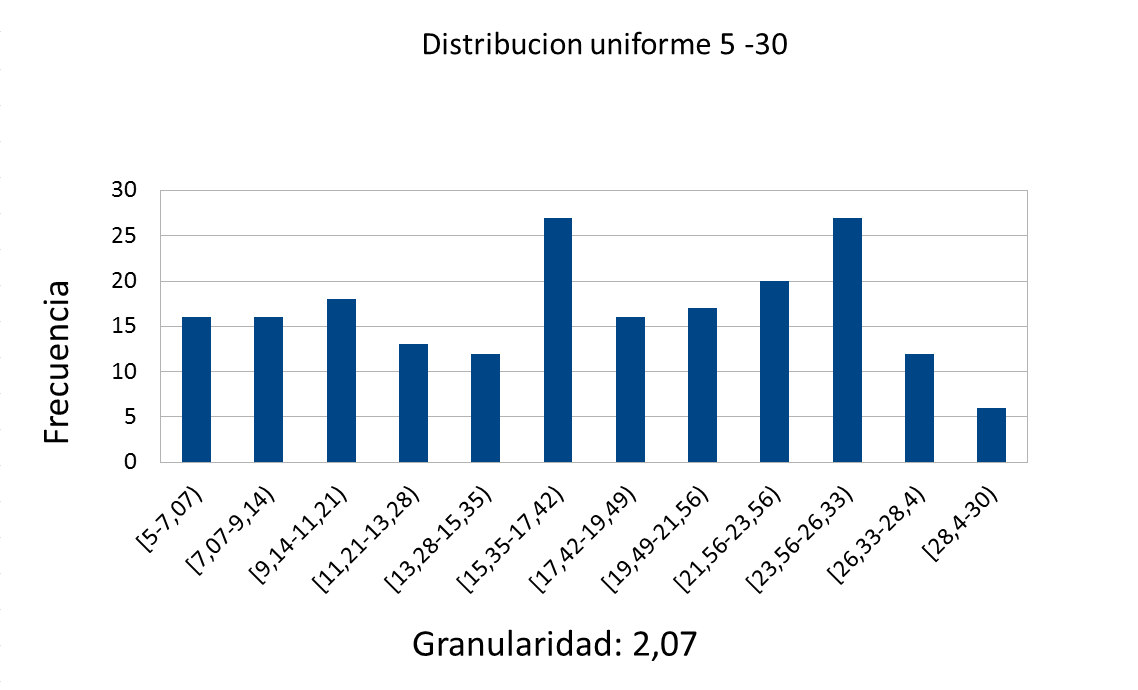
\includegraphics[scale=.40]{imagenes/uniforme_ejemplo.png}
	    \caption{Histograma tiempos de espera de colectivo} 
	    \label{fig:normal_ejemplo1}
	  \end{center}
	\end{figure}

	
\newpage

	\subsection{An\'alisis de los estimadores: Par\'ametro fijo}
			
				\subsubsection*{Caso 1}
		
		\begin{tabular}{| l | l |}
		\hline
		Parametro & 20 \\
		\hline
		Columna & C2 \\
		\hline
		Valor maximo & 1002 \\
		\hline
		Valor minimo & -671 \\
		\hline
		Distribuci\'on & Normal, Media=200 \\
		\hline
		Selectividad de & Igualdad \\
		\hline
		\end{tabular}

		\newpage					

	\begin{figure}[H]
	  \begin{center}
	    %\includegraphics[scale=.41,angle=-90]{imgenes/normal_ejemplo1.png}
	    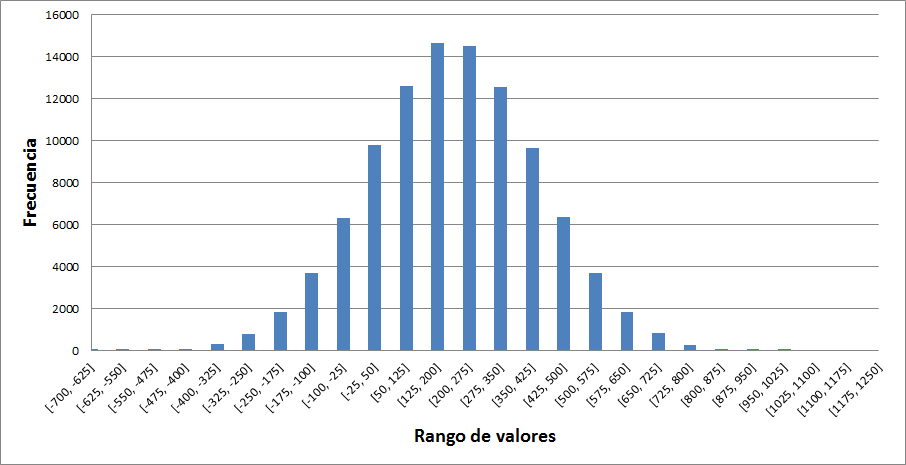
\includegraphics[scale=.40]{imagenes/distro_C2.png}
	    \caption{Grafico de distribucion de la columna C2 del set de datos de la caterda} 
	    \label{fig:(distro_C2}
	  \end{center}
	\end{figure}


	\begin{figure}[H]
	  \begin{center}
	    %\includegraphics[scale=.41,angle=-90]{imgenes/normal_ejemplo1.png}
	    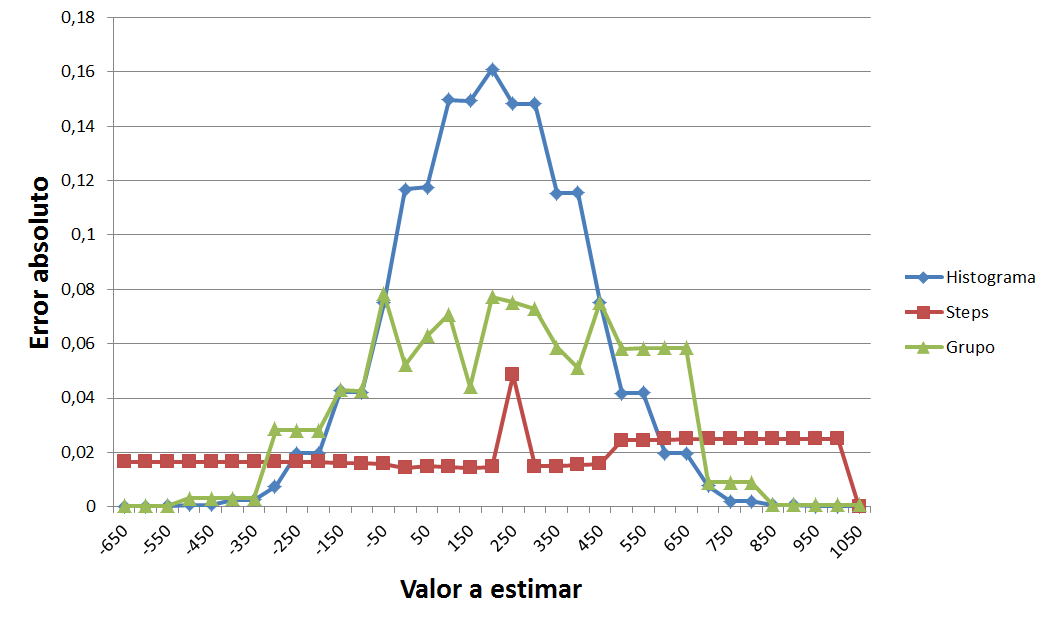
\includegraphics[scale=.40]{imagenes/C2_variando_valor.png}
	    \caption{Errores variando valor a estimar con parametro fijo} 
	    \label{fig:C2_variando_valor}
	  \end{center}
	\end{figure}
		
		En la figura \ref{fig:(distro_C2} se ve la distribucion del set de datos que estamos analizando. Se puede ver como es una distribucion Normal con media 200 y un desv\'io alrededor de 300
		
		En la grafico de la figura \ref{fig:C2_variando_valor} se ve como, teniendo los parametros de los estimadores fijos, y variando el valor a estimar, el estimador de Distribution Steps obtiene un error constante y bastante chico en todo el rango, pero Classic Histogram se comporta mejor en los casos que estan por afuera del desvio standard de la normal (en este caso, al rededor de 300).
		
		Tambi\'en se puede ver como el estimador Classic Histogram obtiene errores muy grandes cuando el valor es muy cercanos a la media. En la media misma se ve como el error llega al m\'aximo.
		
		En cuanto al estimador ideado por el grupo, se ve como al igual que el Histograma, obtiene errores muy chicos en valores lejos del desvio standard de la normal, y a su ves, errores altos en los valores al rededor de la media. Sin embargo, estos errores son inferiores a los obtenidos en el histograma. Esto probablemente se deba a que el estimador de Grupo, es un histograma clasico pero con una re-distribuci\'on en los \textit{bins} con mas valores, los cuales en este caso estarán cerca de la media.
	
		\subsubsection*{Caso 2}
		
		\begin{tabular}{| l | l |}
		\hline
		Parametro & 20 \\
		\hline
		Columna & C0 \\
		\hline
		Valor minimo & 0 \\
		\hline
		Valor maximo & 999 \\
		\hline
		Distribuci\'on & Uniforme, Media = 4950 \\
		\hline
		Selectividad de & Igualdad \\
		\hline
		\end{tabular}		

		\newpage							
	\begin{figure}[H]
	  \begin{center}
	    %\includegraphics[scale=.41,angle=-90]{imgenes/normal_ejemplo1.png}
	    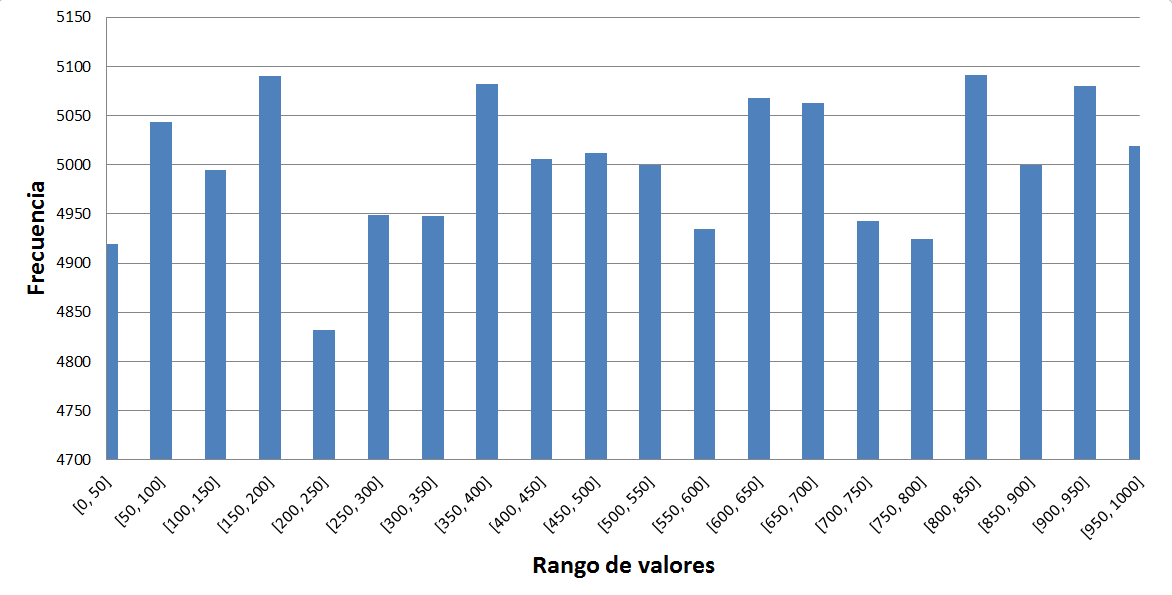
\includegraphics[scale=.50]{imagenes/distro_C0.png}
	    \caption{Grafico de distribucion de la columna C0 del set de datos de la caterda} 
	    \label{fig:(distro_C0}
	  \end{center}
	\end{figure}

	\begin{figure}[H]
	  \begin{center}
	    %\includegraphics[scale=.41,angle=-90]{imgenes/normal_ejemplo1.png}
	    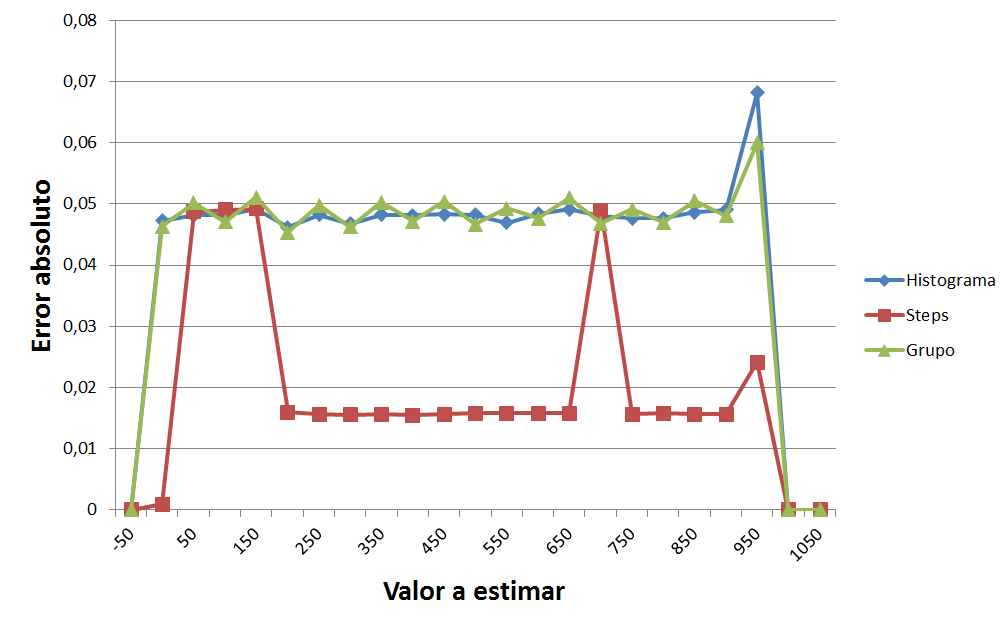
\includegraphics[scale=.40]{imagenes/C0_variando_valor.png}
	    \caption{Errores variando valor a estimar con parametro fijo} 
	    \label{fig:C0_variando_valor}
	  \end{center}
	\end{figure}	

		En la figura \ref{fig:(distro_C0} se ve como la distribucion de los datos esta ves es una Uniforme que varia al rededor de 4950
		
		Segun se ve en la \ref{fig:C0_variando_valor}, no hay una gran diferencia esta ves con el Histograma clasico y el estimador implementado por el grupo. 
		
		En este caso, se puede apreciar como claramente ``Pasos Distribuidos'' obtiene errores bastante menores en casi todo el rango.
		
		Seg\'un pareciera, en los valores donde la distribuci\'on uniforme toma valores altos, los errores de pasos distribuidos aumentan bastante, igualando a los obtenidos en los otros 2 estimadores.

		\subsubsection*{Caso 3}
		
		\begin{tabular}{| l | l |}
		\hline
		Parametro & 20 \\
		\hline
		Columna & C2 \\
		\hline
		Valor maximo & 1002 \\
		\hline
		Valor minimo & -671 \\
		\hline
		Distribuci\'on & Normal, Media=200 \\
		\hline
		Selectividad de & Mayor \\
		\hline
		\end{tabular}

		\newpage					

	\begin{figure}[H]
	  \begin{center}
	    %\includegraphics[scale=.41,angle=-90]{imgenes/normal_ejemplo1.png}
	    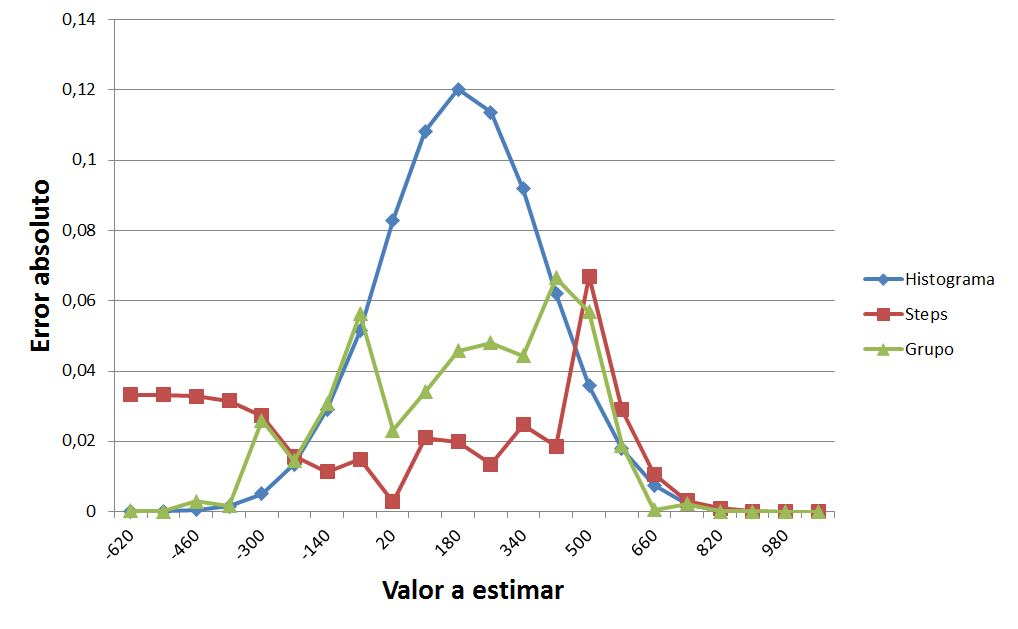
\includegraphics[scale=.40]{imagenes/C2_variando_valor_greater.png}
	    \caption{Errores variando valor a estimar por mayor con parametro fijo} 
	    \label{fig:C2_variando_valor_greater}
	  \end{center}
	\end{figure}
		
		Usando el mismo set de datos uniforme que se uso anteriormente, vemos en la figura \ref{fig:C0_variando_valor_greater} el error de la selectividad pero estimando por mayor. En este caso sucede algo muy parecido a lo que sucede al estimar por menor, con la salvedad de que el de pasos distribuidos no resulta tan constante durante todo el rango.
		
		El error del histograma clasico de nuevo es cada ves mayor a medida que se acerca a la media de la normal. 
		
		El estimador del grupo en esta ocacion resulto ser casi tan bueno como el de pasos distribuidos. Al parecer tiene una buena performance en los datos con distribuci\'on normal.

			\subsubsection*{Caso 4}
		
		\begin{tabular}{| l | l |}
		\hline
		Parametro & 20 \\
		\hline
		Columna & C0 \\
		\hline
		Valor minimo & 0 \\
		\hline
		Valor maximo & 999 \\
		\hline
		Distribuci\'on & Uniforme, Media = 4950 \\
		\hline
		Selectividad de & Mayor \\
		\hline
		\end{tabular}		

	\begin{figure}[H]
	  \begin{center}
	    %\includegraphics[scale=.41,angle=-90]{imgenes/normal_ejemplo1.png}
	    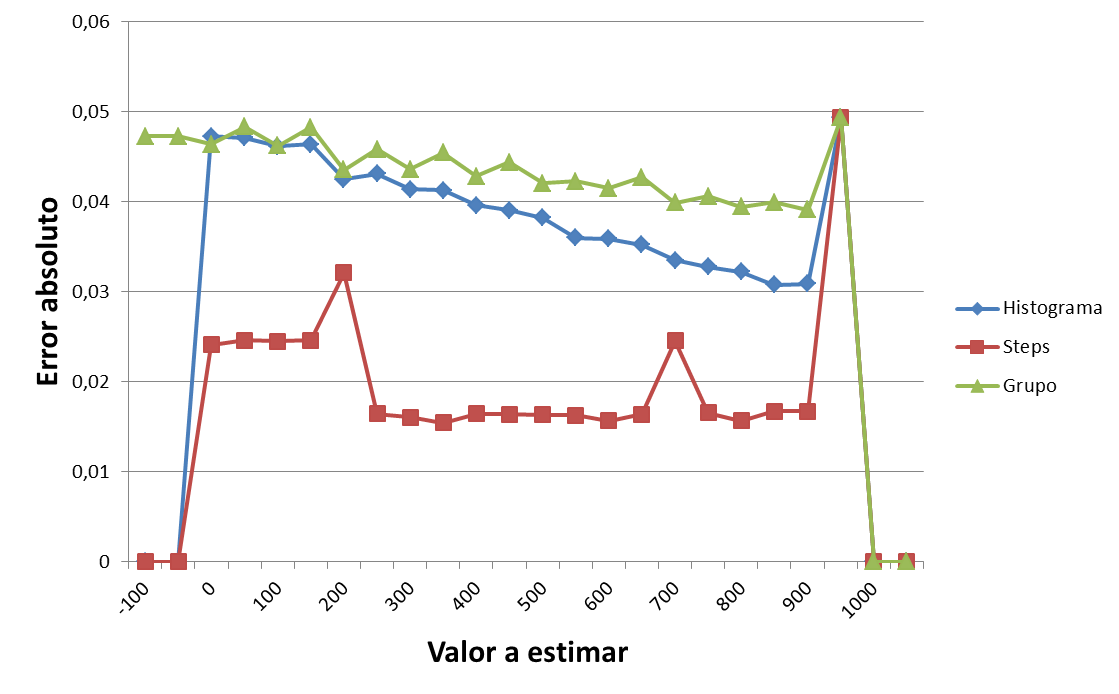
\includegraphics[scale=.40]{imagenes/C0_variando_valor_greater.png}
	    \caption{Errores variando valor a estimar por mayor con parametro fijo} 
	    \label{fig:C0_variando_valor_greater}
	  \end{center}
	\end{figure}	

		En la figura \ref{fig:C0_variando_valor_greater} se realizo un test igual al caso 2, pero esta ves estimando por Mayor enves de por igual. Ya se puede ver como la distribucion es un factor muy importante al momento de utilizar los estimadores.
		
		En este caso, el estimador del grupo fue incluso peor que el histograma clasico, y se ve como la diferencia de error aumenta a medida que se acerca al valor mas alto del rango
	
\newpage
		
	\subsection{An\'alisis de los estimadores: Par\'ametro variable}

		\quad Al igual que en el an\'alisis previo, realizamos mediciones de los estimadores variando el par\'ametro de entrada sobre las mismas poblaciones mencionadas.\\

\quad El par\'ametro que se var\'ia en todos los estimadores representa la cantidad de \textit{buckets}, aunque en el estimador de pasos distribuidos lo llaman \textit{steps}. \\

\quad Se realizaron las comparaciones con un m\'etodo exacto calculado sobre la colecci\'on de datos testeados.

\subsubsection{Distribuci\'on uniforme}

\begin{itemize}
\item \textbf{Operaci\'on por igualdad} \\

\begin{figure}[H]
	  \begin{center}
	    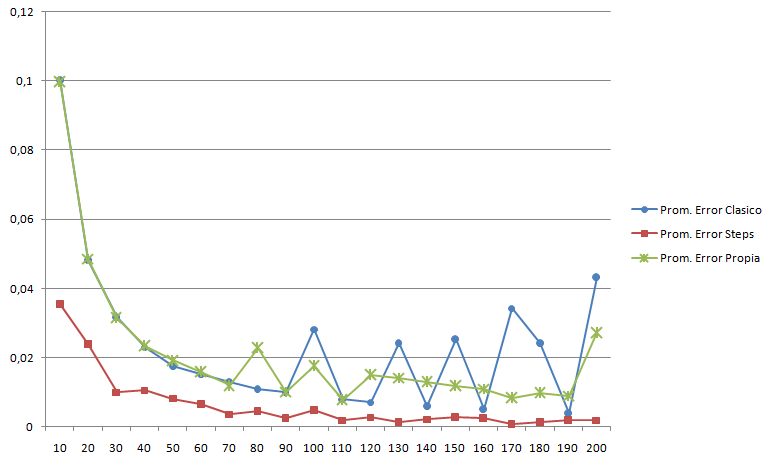
\includegraphics[scale=.80]{imagenes/parametroVariableC0Eq.png}
	    \caption{Error promedio de la Columna C0 de la tabla brindada por la materia} 
	    \label{fig:C0_variando_parametro}
	  \end{center}
\end{figure}

\quad En la figura, se ve claramente como aumentando la cantidad de buckets el error disminuye. Esto se debe a que, al aumentar la cantidad de buckets, se aumenta la granuralidad sobre el rango de valores. Se puede apreciar como para el histograma cl\'asico y el estimador de grupo afecta todav\'ia mucho m\'as que con el de pasos distribuidos. En \'este \'ultimo, al principio mejora bastante (hasta los 70 buckets) pero se estabiliza en un cierto valor y deja de mejorar. En cambio. con los otros dos va mejorando pero se puede ver como se vuelve inestable para ciertos valores del par\'ametro. Creemos que se debe a ciertos casos bordes con respecto a la cantidad de elementos y los valores presentes de un rango y la cantidad de buckets. \\

\item \textbf{Operaci\'on por mayor} \\

\quad Ahora los estimadores los mediremos por su selectividad en un rango buscando ciertos valores en las distribuciones fijos y variando el par\'ametro. \\

\begin{figure}[H]
	  \begin{center}
	    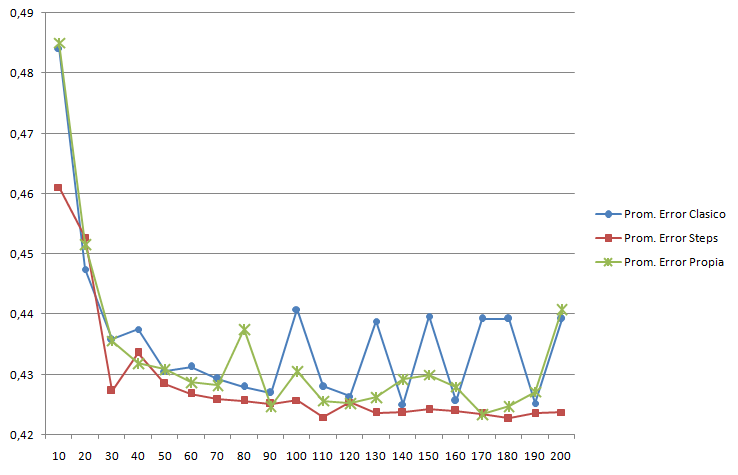
\includegraphics[scale=.80]{imagenes/parametroVariableC0Greater.png}
	    \caption{Error promedio de la Columna C0 de la tabla brindada por la materia} 
	    \label{fig:C0_variando_parametro_greater}
	  \end{center}
\end{figure}

\quad Podemos apreciar la similitudes entre este gr\'afico y el de la Figura	 \ref{fig:C0_variando_parametro}. Pero los valores de error son mucho mayores. \'Esto se debe a que se acumula error, que si bien puede pasar que entre errores se cancelen, creemos que en este caso se acumulan. A pesar de esto, consideramos correcto que mantengan la \textit{forma} ambos gr\'aficos.

\quad Al igual que en el gr\'afico anterior, notamos como el histograma cl\'asico y el estimador propio son inestables. Adem\'as, vuelve a pasar lo mismo con el de pasos distribuidos, mejora hasta cierto punto donde luego de determinado valor del par\'ametro tiende a un valor fijo.

\quad De estos gr\'aficos podemos concluir que para las distribuciones uniformes, el que \textit{mejor} se comporta es el estimador de pasos distribuidos debido a su estabilidad y menor valor de error.

\end{itemize}

\subsubsection{Distribuci\'on normal}

\begin{itemize}
\item \textbf{Operaci\'on por igualdad} \\

\quad Usando la misma metodolog\'ia de tests, analisaremos para colecci\'on de datos con distribuci\'on normal. \\

\begin{figure}[H]
	  \begin{center}
	    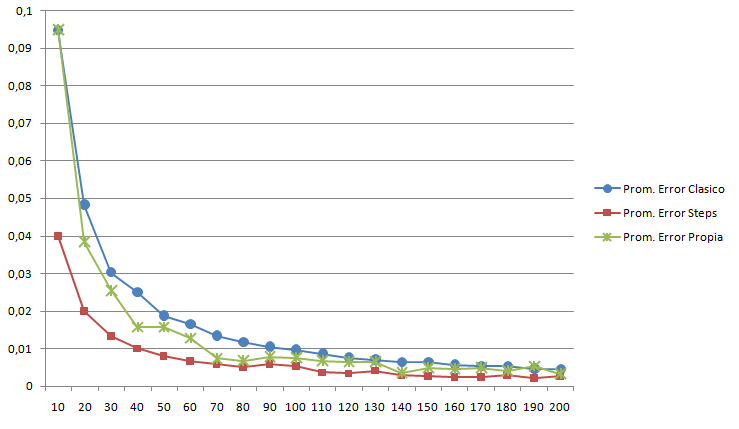
\includegraphics[scale=.80]{imagenes/parametroVariableC2Eq.png}
	    \caption{Error promedio de la Columna C2 de la tabla brindada por la materia} 
	    \label{fig:C2_variando_paremetro}
	  \end{center}
\end{figure}

\quad Nuevamente, todos mejoran a medida de que se aumenta la cantidad de buckets. Pero, en este caso, los tres son estables y, llamativamente, convergen hacia un mismo valor de error. Es decir, que a partir de cierto punto, no hay diferencia apreciable en cuanto al error entre los tres estimadores. Particularmente, cuando la cantidad de buckets es igual a 200, por el gr\'afico se ve que la diferencia entre los estimadores es menor a 0,0025 aproximadamente.\\

\item \textbf{Operaci\'on por mayor} \\

\begin{figure}[H]
	  \begin{center}
	    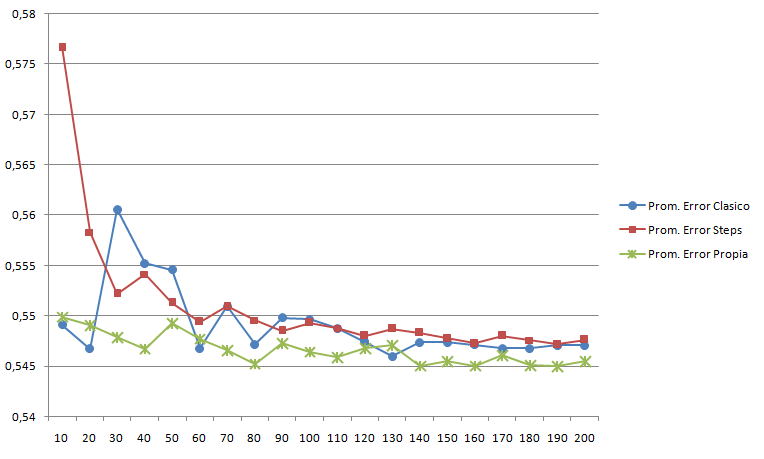
\includegraphics[scale=.80]{imagenes/parametroVariableC2Greater.png}
	    \caption{Error promedio de la Columna C2 de la tabla brindada por la materia} 
	    \label{fig:C2_variando_paremetro_greater}
	  \end{center}
\end{figure}

\quad En esta figura, vemos como el que empieza con mayor error es el de pasos distribuidos y al igual que los otros dos va disminuyendo el error a medida que se incrementa la cantidad de buckets. Con respecto al de histograma cl\'asico, empieza inestable y luego se estabiliza, ocurr\'ia lo contrario en los gr\'aficos \ref{fig:C0_variando_parametro} y \ref{fig:C0_variando_parametro_greater}. En cuanto al estimador propio, vemos que no es tan significativa la mejora compar\'andola con los otros dos pero es el que menor error genera. \\

\quad Se ve que, en este caso, los resultados dieron muy diferentes a todos los anteriores gr\'aficos. Mostrando como, los estimadores dependen del tipo de distribuci\'on y, adem\'as, del tipo de operaci\'on que se realice \\

\end{itemize}
		
	\subsection{An\'alisis para distintas columnas con parametro variable}
	
		\begin{figure}[H]
	    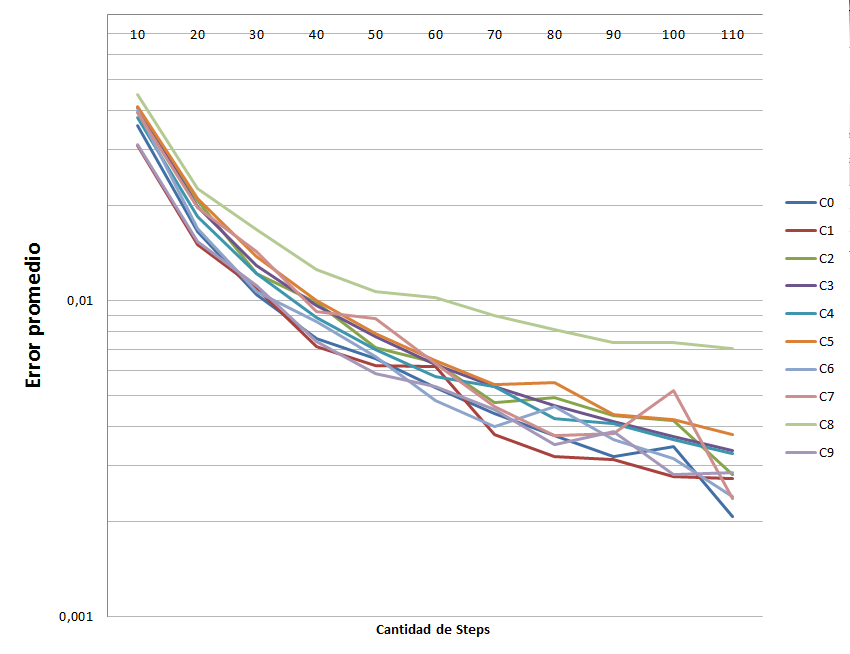
\includegraphics[scale=.60]{imagenes/variacion_parametro_y_columna_steps.png}
	    \caption{Error promedio en Steps para todas las columnas de la tabla brindada por la materia} 
	    \label{fig:variacion_parametro_y_columna_steps}
\end{figure}

	A continuaci\'on, realizamos un an\'alisis del estimador ``Distributed Steps'', el cual obtuvo los mejores resultados seg\'un nuestros an\'alisis previos.
	
	En la figura \ref{fig:variacion_parametro_y_columna_steps} se ve un gr\'afico que se realizo utilizando los errores promedio para cada columna, variando a la ves la cantidad de Steps del estimador y estimando por igualdad. Como error promedio consideramos al promedio de los errores obtenidos para los distintas estimaciones de los valores de una misma columna. Una ves teniendo el error promedio para una cantidad de Steps particular y una columna particular, repetimos el proceso variando la cantidad de Steps para todas las columnas.
	
	Se ve como el error promedio de cada columna, en si es muy similar para pocos Steps, pero al aumentar la cantidad de steps, mejora mucho el error, y esta mejora es bastante independiente de la distribuci\'on de la columna, ya que la diferencia de errores entre columnas, es muy chico.

	Solo para la columna C8 se ve como el error es considerablemente mayor al resto. Esta columna es particularmente distinta a las dem\'as, ya que sus datos van de 0 a 41 y son de una distribuci\'on que no es ni normal ni uniforme, sino que es mas bien como una ``media campana'' con media en el 0, y que va disminuyendo a medida que se acerca al 41, en donde pasa a ser 0. En la archivo ``/tests/Determinar Distribuciones/c8\_distro.xlsx'' se puede ver el gr\'afico del mismo. Sin embargo, por mas de que en esta columna el error haya subido un poco, sigue estando en un valor bastante bajo, por lo que se puede concluir que ``Distributed Steps'' la distribuci\'on de los datos no influye demasiado en el error.
	
	
\begin{figure}[H]
	    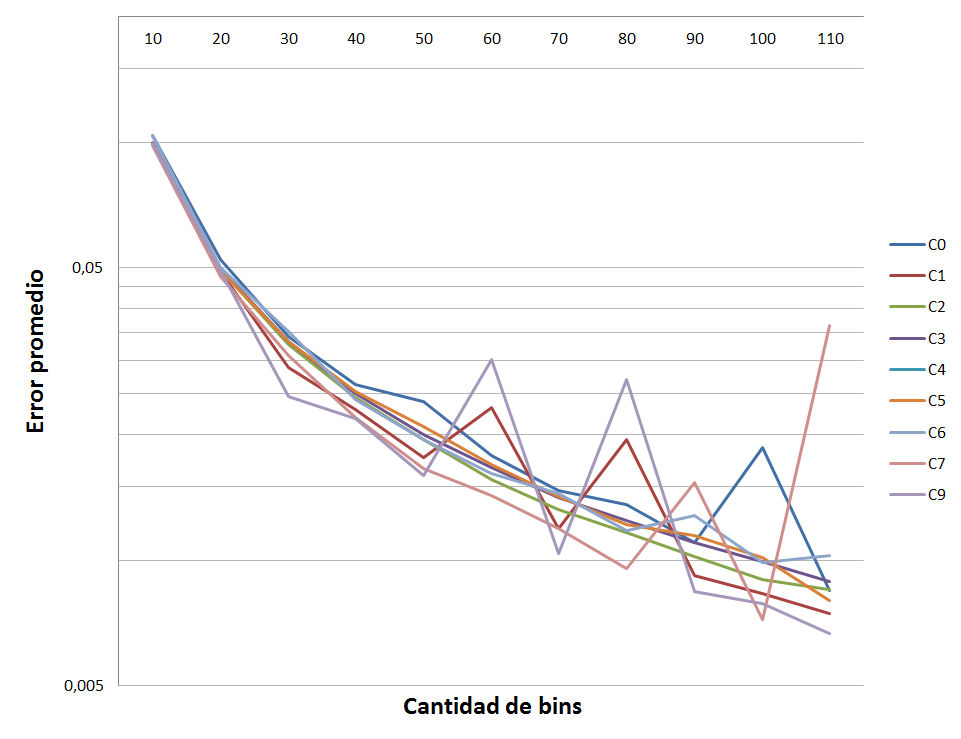
\includegraphics[scale=.60]{imagenes/variacion_parametro_y_columna_histo.png}
	    \caption{Error promedio en Histograma clasico para todas las columnas de la tabla brindada por la materia} 
	    \label{fig:variacion_parametro_y_columna_histo}
\end{figure}

\begin{figure}[H]
	    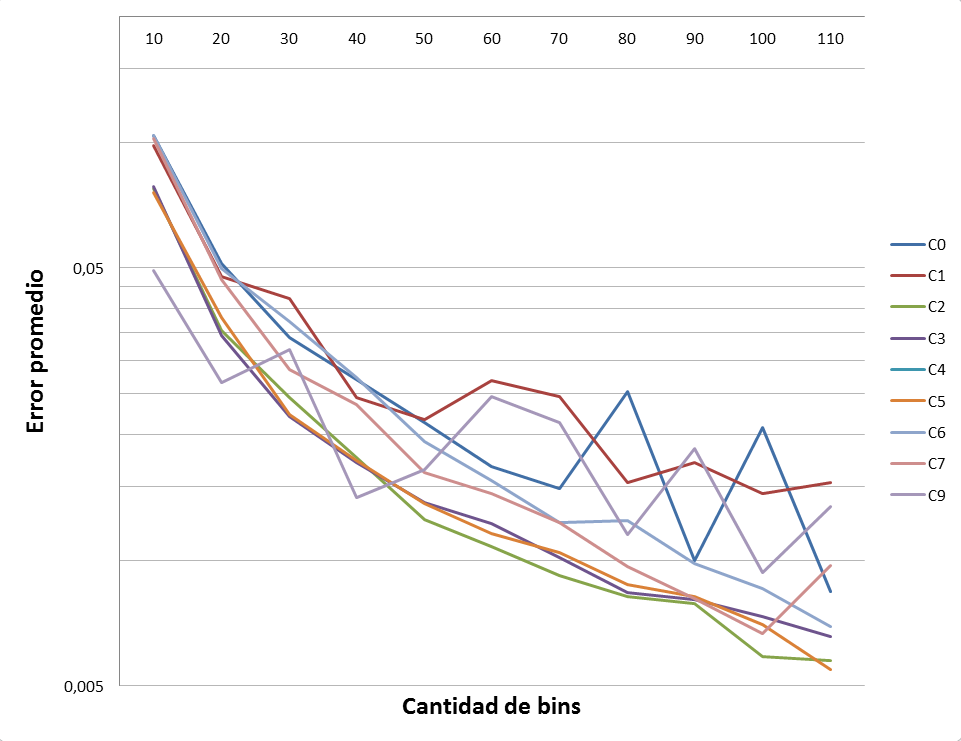
\includegraphics[scale=.60]{imagenes/variacion_parametro_y_columna_grupo.png}
	    \caption{Error promedio en Estimador del grupo para todas las columnas de la tabla brindada por la materia} 
	    \label{fig:variacion_parametro_y_columna_grupo}
\end{figure}

Adicionalmente, se puede ver en las figuras \ref{fig:variacion_parametro_y_columna_histo} y \ref{fig:variacion_parametro_y_columna_grupo} el mismo analisis realizado para Steps, pero esta ves para Histograma cl\'asico y el estimador echo por el grupo respectivamente. En estos graficos no se incluyo la columna C8, ya que la misma tiene datos que del 0 al 41, por lo que tienen un rango de 41, y para 50 buckets se tiene 1 bucket para cada valor, por lo que el error pasa a ser 0.

	Compar\'andolos con el gr\'afico de Steps, a primera vista se ve como en general Steps se comporta mejor considerando un valor del par\'ametro fijo. 
	
	A diferencia del de steps, el histograma cl\'asico no es tan independiente de la distribuci\'on de los datos, se puede ver como para las distintas columnas el error var\'ia bastante. 
	
	En cuanto al estimador del grupo, lo que se puede apreciar es que para algunas columnas, se comporta mejor que el Histograma cl\'asico, y dif\'icilmente se comporta mejor que Steps. Debido a lo analizado anteriormente, sabemos que el estimador del grupo tenia una mejor performance sobre el cl\'asico solo en las distribuciones normales, y en las uniformes los errores no variaban mucho entre uno y otro. Las columnas donde la performance es mejor que en el histograma, son las C2, C3 y C5. En el anexo a este informe, en la carpeta "/tests/Determinar Distribuciones" se encuentran los gr\'aficos de las columnas mencionadas. No fueron incluidos en este informe, debido a que eran demasiados y nos iban a quedar demasiados gr\'aficos. Tambien se encuentran graficadas las distribuciones de las columnas C1 y C9, que son las que obtuvieron errores mayores.
	
	En esos gr\'aficos, se puede ver como las distribuciones de esas columnas C2, C3 y C5 son todas normales, y C1 y C9 son de otra distribucion muy distinta, que no es normal ni uniforme, por lo que se puede comprobar que nuestro an\'alisis previo, en donde nuestro estimador se comportaba mejor en distribuciones normales, es correcto.
	
		
\end{document}